\documentclass{imammb}
\jno{dqnxxx}
\usepackage[english]{babel}
\usepackage[pagebackref=true]{hyperref}
\usepackage{doi}
\usepackage{amsmath, amsthm, bm, mathrsfs}
% %%%%%%%%%%%%%%%%%%%%proof
%
\renewenvironment{proof}[1][Proof]{\noindent\textit{#1. } }{\hfill$\square$}



%%%%%%%%%%%%%%%%Dcolumn 

%!TEX root = ./main.tex



 \newtheoremstyle{theorem}{6pt}{6pt}{\rm}{}{\sffamily}{ }{ }{}
 \theoremstyle{theorem}
\newtheorem{theorem}{\sc Theorem}[section]

 \newtheoremstyle{algorithm}{6pt}{6pt}{\rm}{}{\sffamily}{ }{ }{}
 \theoremstyle{algorithm}
\newtheorem{algorithm}{\sc Algorithm}[section]



 \newtheoremstyle{lemma}{6pt}{6pt}{\rm}{}{\sffamily}{ }{ }{}
 \theoremstyle{lemma}
 \newtheorem{lemma}{\sc Lemma}[section]


\newtheoremstyle{case}{6pt}{6pt}{\rm}{}{\sffamily}{. }{ }{}
 \theoremstyle{case}
\newtheorem{case}{{\sc Case}}

 \newtheoremstyle{statement}{6pt}{6pt}{\rm}{}{\sffamily}{ }{ }{}
\theoremstyle{statement}
\newtheorem{statement}{\sc Statement}

 \newtheoremstyle{corollary}{6pt}{6pt}{\rm}{}{\sffamily}{ }{ }{}
 \theoremstyle{corollary}
 \newtheorem{corollary}{\sc Corollary}[section]
 
  \newtheoremstyle{definition}{6pt}{6pt}{\rm}{}{\sffamily}{ }{ }{}
 \theoremstyle{definition}
 \newtheorem{definition}{\sc Definition}[section]
 
\newtheorem{acknowledgement}[theorem]{Acknowledgement}

\newtheorem{axiom}[theorem]{Axiom}

\newtheorem{claim}[theorem]{Claim}
\newtheorem{conclusion}[theorem]{Conclusion}
\newtheorem{condition}[theorem]{Condition}
\newtheorem{conjecture}[theorem]{Conjecture}
\newtheorem{criterion}[theorem]{Criterion}


\newtheoremstyle{example}{6pt}{6pt}{\rm}{}{\sffamily}{ }{ }{}
\theoremstyle{example}
\newtheorem{example}[theorem]{\sc Example}

\newtheorem{exercise}[theorem]{Exercise}

\newtheorem{notation}[theorem]{Notation}
\newtheorem{problem}[theorem]{Problem}




\newtheoremstyle{remark}{6pt}{6pt}{\rm}{}{\sffamily}{ }{ }{}
\theoremstyle{remark}
\newtheorem{remark}{\sc Remark}[section]
\newtheorem{solution}[theorem]{Solution}
\newtheorem{summary}[theorem]{Summary}
\newtheoremstyle{approximation}{6pt}{6pt}{\rm}{}{\sffamily}{ }{ }{}
\theoremstyle{approximation}
\newtheorem{approximation}{\sc Approximation}




\newtheoremstyle{scheme}{6pt}{6pt}{\rm}{}{\sffamily}{ }{ }{}
\theoremstyle{scheme}
\newtheorem{scheme}{\sc Scheme}

\newtheoremstyle{Algorithm}{6pt}{6pt}{\rm}{}{\sffamily}{ }{ }{}
\theoremstyle{Algorithm}
\newtheorem{Algorithm}[theorem]{\sc Algorithm}



 
\newtheoremstyle{Assumption}{6pt}{6pt}{\rm}{}{\sffamily}{ }{ }{}
\theoremstyle{Assumption}
\newtheorem{Assumption}{\sc Assumption}[section]


\newtheoremstyle{proposition}{6pt}{6pt}{\rm}{}{\sffamily}{ }{ }{}
\theoremstyle{proposition}
\newtheorem{proposition}{\sc Proposition}[section]





\newtheoremstyle{hypo}{6pt}{6pt}{\rm}{}{\sffamily}{ }{ }{}
 \theoremstyle{hypo}
 \newtheorem{hypo}{\sc Hypothesis}[section]
 
  \newtheoremstyle{Step}{6pt}{6pt}{\rm}{}{}{ }{ }{}
 \theoremstyle{Step}
\newtheorem{Step}{Step}

 

\usepackage{bbold}
\usepackage{booktabs}
\usepackage{graphicx}
\usepackage[utf8]{inputenc}
\usepackage[T1]{fontenc}
\usepackage{caption}
\usepackage{siunitx}
\usepackage{xspace}
\usepackage{color}
\usepackage{proba}
\usepackage{natbib}

\usepackage[usenames,dvipsnames,svgnames,table]{xcolor}
\usepackage{cleveref}
\usepackage{paralist}
% \usepackage[disable]{todonotes}
\usepackage[textwidth=1in, textsize=tiny]{todonotes}
\usepackage{bigints}
\usepackage[title,titletoc,toc]{appendix}
\usepackage{siunitx}
\usepackage{acro}
\oddsidemargin=1cm
\textwidth=14.5cm
\DeclareMathAlphabet{\mathpzc}{OT1}{pzc}{m}{it}
\newtheorem{dfn}{Definition}
\newtheorem{thm}{Theorem}[section]
\newtheorem{pro}{Proposition}[section]
\newtheorem{lem}{Lemma}[section]
\newtheorem{definition}{Definition}[section]
\newtheorem{corollary}{Corollary}[section]
\newtheorem{consequence}{CONSEQUENCE}[section]
\newtheorem{remark}{Remark}[section]
\newtheorem{example}{\bf Example}[section]
\newtheorem{proof}{\bf Proof}[section]
\newtheorem{assumption}{Assumption}[section]
\newproof{pf}{Proof}
\newproof{Proof}{Proof}
\providecommand*{\lemautorefname}{Lemma}
\providecommand*{\thmautorefname}{Theorem}
\providecommand*{\assumptionautorefname}{Assumption}

\newcommand{\fin}{\vrule height3pt width3pt depth2pt}
\newcommand{\normL}[1]{\left[\mathbb{E}\left|#1\right|^2\right]^{1/2}}
\newcommand{\ms}[1]{\mathbb{E}\left|#1\right|^2}
\newcommand{\mep}[1]{\mathbb{E}|#1|^p}
\newcommand{\m}[1]{\mathbb{E}#1}
\newcommand{\Prob}[1]{\mathbb{P}\left[#1\right]}
\newcommand{\meanp}[2]{\mathbb{E}\left|#1\right|^{#2}}
\newcommand{\condexp}[2]{\mathbb{E}\left[#1|#2\right]}
\newcommand{\lftrght}[3]{\left#2 #1\right #3}\DeclareMathOperator{\tr}{tr}
\newcommand{\innerprod}[2]{\left\langle#1, #2\right\rangle}
\newcommand*{\eg}{e.g.,\xspace}
\newcommand*{\ie}{i.e.,\xspace}
%\newcommand*{\todo}[1]{\textcolor{BrickRed}{#1}\\}
\newcommand{\crefrangeconjunction}{--}
\crefrangeformat{equation}{(#3#1#4)--(#5#2#6)}
\DeclareMathOperator{\diag}{diag}
\DeclareMathOperator*{\as}{a.s.}
%
\DeclareAcronym{DENV-1}{
	short = DENV-1 ,
	long = Dengue Virus Serotype 1
}
\DeclareAcronym{DENV-2}{
	short = DENV-2 ,
	long = Dengue Virus Serotype 2
}
%
\DeclareAcronym{ADE}{
	short = ADE,
	long = Antibody Dependent infection Enhancement
}
\DeclareAcronym{DCF}{
	short = DCF ,
	long = Dengue Classic Fever
}
\DeclareAcronym{DHF}{
	short = DHF ,
	long = Dengue Hemorrhagic Fever
}


\newcommand{\tinytodo}[2][]
{\todo[caption={#2}, size=\tiny, #1]{
	\renewcommand{\baselinestretch}{0.5}\selectfont#2\par}
}
\renewcommand{\theequation}{\thesection.\arabic{equation}}
\numberwithin{equation}{section}
\def\citeasnoun{\cite}
%
\begin{document}
% 	%\title{
		Modeling and $R_0$ estimation  of the 2010 Dengue Hemorrhagic Fever 
        Outbreak in Hermosillo Sonora.
%\tnoteref{t1}
}%,t2}}
%\tnotetext[t1]{
%	This work has been partially
%	supported by CONACYT project *****
%}
\author[conacyt-unison]{S. D\'{\i}az-Infante \corref{cor1}}
\ead{saul.diazinfante@unison.mx}
%
\author[unison]{J. A. Montoya Laos}
%\ead{montoya@unison.mx}
%
\author[unison]{D. Olmos Liceaga}
%\ead{daniel.olmos@unison.mx}
%
\author[colson]{P. A. Reyes Castro}
%\ead{preyes@colson.edu.mx}
\author[colson]{A. L. Castro Luque}

\address[conacyt-unison]{
	CONACYT-Universidad de Sonora,
	Departamento de Matem\'aticas, Universidad de Sonora\\
	Blvd. Rosales y Luis Encinas S/N, Col. Centro, Hermosillo, Sonora, C.P. 83000,
	M\'exico\\
}
%
\address[unison]{
	Departamento de Matem\'aticas, Universidad de Sonora\\
	Blvd. Rosales y Luis Encinas S/N, Col. Centro, Hermosillo, Sonora, C.P. 83000,
	M\'exico\\
}
%
\address[colson]{
	Centro de Estudios en Salud y Sociedad,
	El Colegio de Sonora, Avenida Obregón No. 54, Colonia Centro, C.P. 83000,
	Hermosillo, Sonora. México
}
%
\cortext[cor1]{Corresponding author}
\begin{abstract}
	We model and estimate the basic reproductive number of Dengue  and 
	Dengue Hemorrhagic Fever outbreak of the 2010 from Hermosillo Sonora.
	Our results suggest that serotype DENV-2 of the Dengue virus and the cross 
    infection risk enhancement hypothesis, could explain the incidence of
    Dengue Hemorrhagic Fever cases reported by Secretaria de Salud del Estado de 
    Sonora.
\end{abstract}
\begin{keyword}
	Differential Equations;
	Dengue Hemorrhagic Fever;
	Boot strap;
\end{keyword}
\journal{Epidemics}
     \today
     \section{Introduction} \label{intro}
         State the objectives of the work and provide an adequate 
         background, avoiding a detailed literature survey or a 
         summary of the results.
% %
         \paragraph{Objectives}
         Our objective is to explain the dengue hemorrhagic outbreak that 
      occurred in the city of Hermosillo, Sonora in2010.
%     %
     \paragraph{Severity}
     \ac{DCF} 
     \ac{DHF} description.
     \paragraph{ADE hypothesis}
      sequence and
      \\
      \ac{DENV-1}, \ac{DENV-2}
      reinfection as cause of hemorrhagic.
         \paragraph{Background}
       
     \section{Material and methods}
         Provide sufficient detail to allow the work to be 
         reproduced, with details of supplier and catalogue 
         number when appropriate. Methods already published 
         should be indicated by a reference: only relevant 
         modifications should be described.
         \subsection{Data}
             \paragraph{Data description (Pablo)}
            	\input{data_description.tex} % Pablo
             \paragraph{Socioeconomic description: 
                 homogeneity of regarding initial
                 grow geographic area (Ana-Lucia)}
         %!TEX root = ./main.tex
 % Ana-Lucia
         \subsection*{Model}
             %\paragraph{Introduction}
    Our work aims to explain the \ac{DHF} cases reported in the Hermosillo's 
2010 outbreak. Thus, our formulation only considers the time of the epidemic and
supposes that at this period, the \ac{DENV-2} serotype invades for the first 
time the city. We understand the\ac{DHF} cases as a consequence of reinfection 
with the \ac{DENV-2} serotype. That is, a fraction of individuals with immunity 
to serotype \ac{DENV-1}\textemdash acquired by past outbreaks\textemdash 
increments their susceptibility to the \ac{DENV-2}, and consequently 
develops hemorrhagic with a certain probability.

             %The model we consider in this work has the following hypothesis. We 
%consider that mosquitoes are present in the medium and their presence has 
%an asymptotic growth. In many situations it has been considered that
%mosquitoes vary respect the climatological conditions. Moreover in some work 
%there has been studies where mosquitoes densities change periodically following 
%a periodic time dependent birth rate. However, our interest is to consider 
%the dynamics for the rain season for one year.
%
%	Our study focuses on a dengue outbreak that occurred on 2010 in the 
%city of Hermosillo. It was reported that in that year there was circulating one 
%serotype different from the 2. The presence of a second serotype was reported
%to occur on year 2011? However, as for 2010, there was a significant presence 
%of \ac{DHF} cases, it lead us to assume that 2010 was the year that serotype 2
%arrived to Hermosillo.
%
%	For our model we do not consider an exposed class. For our model a fraction 
%$\theta$ of the humans in class $S_1$ that are bitten by a mosquito of serotype 
%2 are the hemorrhagic cases. The rest of such cases belong to the classic
%version of the disease.
%
 % Daniel
             %!TEX root = ./main.tex
\section*{Important Hypothesis (Daniel-Saúl)}
    \paragraph{Permanent immunity}
    Accordingly to \cite{WHO}, Dengue infection caused by a DEN-i serotype induces long-life immunity to reinfection for this strain. Also,  a recovered individual previously infected with DEN-i Dengue serotype, acquires partial immunity to a different serotype for about a period of two years \cite{Reich2013}. As our study focuses on a single year dynamics, we assume that a susceptible individual who has never get infected before, could obtain Dengue by any of serotypes DENV-1, or DENV-2, and then becoming recovered to any strain for the rest of the year. 
    
    %
    \paragraph{ADE hypothesis}
    The processes and factors that produce \ac{DHF} are still unclear. Different factors have
    been observed to be responsible for DHF \cite{Martina2009}. However, one of the most predominant hypothesis claims that reinfection with a different serotype enhances the probability of developing plasma vascular permeability---the \ac{ADE} hypothesis \citep[see, e.g.][p. 295]{Halstead1992}, \cite{Guzman2013}. We consider in our formulation the ADE hypothesis, that 
    is, only a fraction of the second reinfection with serotype \ac{DENV-2} develops vascular leaking. Additionally, a second consequence of the ADE hyphotesis, is that the susceptibility of acquiring dengue a second time, is increased \cite{Recker2009}. \\
    %But there also exist studies that report first infection DHF cases \cite{Debast1993}.
%
    \paragraph{\ac{DENV-2} report circulation in Hermosillo}
    According to \cite{Vazquez2011} and \cite{Reyes2017}, in year 2010 only DENV-1 was confirmed to be present in the state of Sonora. In contrast, even there is currently presence of DENV-2 in the state, due to limited serotyping of cases it is not clear when DENV-2 began circulating the state \cite{Reyes2017}. In order to argue that reinfection with DENV-2 might have been responsible for DHF, we follow previous studies, such as the work by \cite{Gomez2014} and \cite{Vazquez2011}. In \cite{Gomez2014}, the authors analyze the dengue situation in Mexico for the period 2000 to 2011, and argue that the increase of DHF in 2001 in Yucat\'an was linked to the introduction of the DENV-2 strain. 
    On the other hand DENV-2 was reported to be present in Sinaloa and Baja California Sur in 2009 \cite{Vazquez2011}, which are neighbor states of Sonora. These studies support our hypothesis that DHF in 2010 in Hermosillo, was due to the introduction of DENV-2 into the state of Sonora. 
    
    \paragraph{Asymptomatic and reported cases} In order to estimate the solution that best fit the 
    evolution of the number of reported cases, we utilize a fraction $p$ of the individuals that our model identifies as DCF cases. Such fraction is based on two factors (i) The proportion of asymptomatic cases respect to the total infected individuals, which ranges from the $75\%$ to the $80\%$ (\cite{Bosch2018}, \cite{Reiter2010}) and (ii) from the symptomatic cases, only a fraction of them
     go to the hospital, and the test for DEN-V is taken. 
    
%    On the other hand, reported cases represent only a fraction of the infected individuals obtained by the model. Then, our data is compared to a fraction of individuals that belong to the first and second time infected classes.
%    We assume that the $X\%$ (pending) of the \ac{DCF} are asymptomatic, whereas for 
%    \ac{DHF}  all the cases are reported. 
    
    
%    Therefore, the class $Y_{-1}^{[h]}$ accounts for
%    all the \ac{DHF} cases, whereas a fraction $p=0.05$ of the sum 
%    $I_1+ I_2 + Y_{-1}^{[c]}$ represent the confirmed cases of \ac{DCF}. (75\% is the amount of asymptomatic according to literature)

    \tinytodo{Incluir citas de los 
        porcentages de asintomáticos,
        http://www.who.int/%
        en/news-room/fact-sheets/%
        detail/dengue-and-severe-dengue %
        says that about% 
        75$\%$ is asymptomatic}

    \todo{chastel2012.pdf}
    
    \paragraph{Homogeneity about the early outbreak stage}
In this model    
    

    \paragraph{Vector transmission dynamics}
        Define the infection forces as
    \begin{equation}
        \begin{aligned}
            A_{I_1} &=
                \frac{\beta_Mb}{N_H} I_1, \qquad
            A_{I_2}=
                \frac{\beta_Mb}{N_H} I_2,
        \\
            A_{Y_{-1}^{[h]}}&=
            \frac{\beta_Mb}{N_H} Y_{-1} ^{[h]}, \qquad
            A_{Y_{-1}^{[c]}}=
                \frac{\beta_Mb}{N_H} Y_{-1}^{[c]},
        \\
            B_{M_1} &= 
                \frac{\beta_Hb}{N_H}M_1, \qquad
            B_{M_2}=
                \frac{\beta_Hb}{N_H}M_2 ~.
        \end{aligned}
    \end{equation}

    Define
    $$
        A_{\bullet}:=
            A_{I_1} + A_{I_2} + A_{Y_{-1}^{[h]}} + 
            A_{Y_{-1}^{[c]}}
    $$
    as the total human infection force, that is, 
    the sum of all
    human contributions to the vector infection. 

    Then we describe the mosquito disease dynamics 
    by 
    \begin{equation}
        \begin{aligned}
            \\
            \frac{dM_S}{dt}&=
                \Lambda_M
                - A_{\bullet} M_S
                - \mu_M M_S
            \\
            \frac{dM_1}{dt}&=
                A_{I_1}  M_S - \mu_M M_1
            \\
            \frac{dM_2}{dt} &=
                \left(
                    A_{I_2}+A_{Y_{-1}^{[h]}}+A_{Y_{-1}^{[c]}}
                \right) 
                M_S-\mu_M M_2
        \end{aligned}
    \end{equation}
    Here $M_S$, is the vector susceptible class and
    $M_1$, $M_2$ respectively denotes the vector 
    Infected classes with \ac{DENV-1}
    and \ac{DENV-2}. 
    
    
    
    \paragraph{Host disease dynamics}
        Susceptible individuals ($S$) become infected for the first time
        with DENV-1 or DENV-2 after a successful mosquito bite and move
        to classes $I_1$ and $I_2$, respectively. Individuals in these classes can 
        be symptomatic or asymptomatic. From \cite{Bosch2018}, we know that asymptomatic 
        individuals are able to transmit the disease with an $80\%$ of effectiveness, compared 
        to symptomatic cases. Therefore, our model, makes no distinction between symptomatic and asymptomatic individuals for the disease dynamics.  
        After $\alpha_c^{-1}$ time units,. infected individualsFrom here, they remain
        in the infected class for $1/\alpha_c$ time units, after which,
        move to a recovered class $R_S$.  
        As we are interested in a one
        year dynamics, for the rest of the epidemic they become immune to
        any serotype. A second class of susceptible individuals $S_{-1}$,
        consist on those who acquired DENV-1 in previous years and in the
        current year are susceptible only to DENV-2. Such individuals
        become infected with DENV-2 when exposed to infected mosquitoes
        with that serotype. It is worth mentioning that asymptomatic individuals are 
        able to transmit the disease with an $80\%$ of effectiveness, compared 
        to symptomatic cases \cite{Bosch2018}. Therefore, our model, makes no 
        distinction between symptomatic and asymptomatic individuals for the disease dynamics. 
    
        
        In \cite{OhAinle2011} and
        \cite{Sangkawibha1984} it was observed that a more severe version
        of dengue occurs (might occur?) when an individual acquires dengue
        for a second time, and this happens to be DENV-2. Based on this
        assumption, an individual from $S_{-1}$ moves to $Y_{-1}^{[c]}$ or
        $Y_{-1}^{[h]}$, if the infection leads to DCF or DHF, respectively.
        Finally, these infected individuals move to the recovered class
        $R_{S_{-1}}$ at rates $\alpha_c$ and $\alpha_h$, respectively. For
        our model, $\mu_H$ is the human death rate; $b$ is the number of
        bites per week per mosquito and $\beta_H$ is the effectiveness of
        the bite. From the current hypothesis our model is given by    

%Assuming sufficient density of vectors, we 
%describe the \ac{DCF} and \ac{DHF},
%using a cross infection mechanism similar to the 
%reported in \cite{Feng1997a}. 
%Our version allows a hemorrhagic description of 
%the Infected human population 
%with serotype $i$---see 
%\Cref{tbl:variable_description,tbl:parameter_description}
%to variable and parameter description. The symbol 
%$I_{i}$ represents the human infected 
%pupulation with serotype $i$,
%which never was infected before, while 
%$Y_{-i}^{[\star]}$ denotes the 
%number of humans which are immune to serotype 
%$i$ at the time of the 
%present outbreak and develops dengue of type 
%$\star$ (DCF or DHF).
%Then $S_{-i}$ are the individuals who were 
%infected with serotype $i$ in the 
%previous outbreak, and at the current time, are 
%susceptible only to a serotype different of $i$.
%Dengue cross infection.

\begin{equation}\label{eqn:model_two_strains1}
    \begin{aligned}
        \frac{dS}{dt} &=
            \mu_HN_S - (B_{M_1} + B_{M_2}) S
            -\mu_H S
        \\
        \frac{dI_1}{dt} &=
            B_{M_1} S
            -(\alpha_c + \mu_H) I_1
        \\
        \frac{dI_2}{dt} &=
            B_{M_2} S
            -(\alpha_c + \mu_H)I_2
        \\
        \frac{dR_S}{dt}&=\alpha_c (I_1+I_2)-\mu_H R_S
        \\
        \frac{dS_{-1}}{dt} &=
            \mu_HN_{S_{-1}}- \sigma B_{M_2} S_{-1}-\mu_H S_{-1}
        \\
        \frac{dY_{-1} ^{[c]} }{dt} &=
            (1 - \theta) \sigma B_{M_2} S_{-1}
            -(\alpha_c + \mu_H) Y_{-1} ^ {[c]}
        \\
        \frac{dY_{-1}^{[h]}}{dt} &=
            \theta \sigma B_{M_2} S_{-1}
            -(\alpha_h + \mu_H)Y_{-1} ^{[h]} 
        \\
        \frac{dR_{S_{-1}}}{dt} &= 
            \alpha_c Y_{-1} ^{[c]}
            + \alpha_h Y_{-1} ^ {[h]} - \mu_H R
    \end{aligned}
\end{equation}
    Here, we take $N_H=N_S+N_{S_{-1}}$ as the total number of individuals.
    For our formulation $N_H, N_S$ and $N_{S_{-1}}$ remain constant. $N_S$
    is the total number of individuals that are involved in the first
    infection dynamics ($N_S = S +I_1+I_2+R_S$). On the other hand
    $N_{S_{-1}}$ is the total number of individuals involved in the
    reinfection dynamics ($N_{S_{-1}}=S_{-1}+Y_1^{[c]}+
    Y_1^{[h]}+R_{S_1}$). Also, the recovered individuals in both classes
    can be considered as a single recovered class $R=R_S+R_{S_{-1}}$ as
    our dynamics are taken only for one year. Then, our equations become

\begin{equation}\label{eqn:model_two_strains2}
    \begin{aligned}
        \frac{dS}{dt} &=
            \mu_H N_S - (B_{M_1} + B_{M_2}) S
            -\mu_H S
        \\
        \frac{dI_1}{dt} &=
            B_{M_1} S
            -(\alpha_c + \mu_H) I_1
        \\
        \frac{dI_2}{dt} &=
            B_{M_2} S
            -(\alpha_c + \mu_H)I_2
        \\
        \frac{dS_{-1}}{dt} &=
            \mu_HN_{S_{-1}}- \sigma B_{M_2} S_{-1}-\mu_H S_{-1}
        \\
        \frac{dY_{-1} ^{[c]} }{dt} &=
            (1 - \theta) \sigma B_{M_2} S_{-1}
            -(\alpha_c + \mu_H) Y_{-1} ^ {[c]}
        \\
        \frac{dY_{-1}^{[h]}}{dt} &=
            \theta \sigma B_{M_2} S_{-1}
            -(\alpha_h + \mu_H)Y_{-1} ^{[h]} 
        \\
        \frac{dR}{dt} &= 
            \alpha_c 
                \left(
                    I_1 + I_2 + Y_{-1} ^{[c]}
                \right)
            + \alpha_h Y_{-1} ^ {[h]} - \mu_H R
    \end{aligned}
\end{equation}


\todo{Fix $\Lambda _{\cdot} = N$. }
\todo{Include information about the 2 strains}
\begin{figure}[htb]
	\centering
	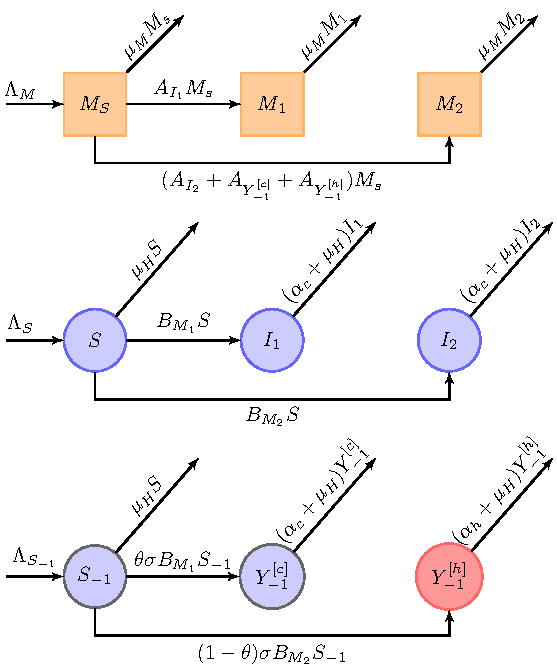
\includegraphics[width=\linewidth]{disiase_flow.pdf}
	\caption{Flow diagram of model \eqref{eqn:model_two_strains}}.
	\label{fig:disiaseflow}
\end{figure}
%
\begin{table*}[h!]
	\begin{center}
		\begin{tabular}{rl}
			\toprule
			Symbol		&	\multicolumn{1}{c}{Meaning}
			\\
			\midrule
			$M_S$
				& Number of susceptible mosquitoes.
			\\
			$M_1$, $M_2$
				&
				 Number of infected mosquitoes with virus
				\\
				& 
				serotype \ac{DENV-1} or \ac{DENV-2}.
			\\
			$S$
				&
				Susceptible host population which, 
				\\
				& never has acquired dengue.
			\\
			$S_{-1}$
			&
				Susceptible host population 
				which is immune to
			\\
			&
				serotype $1$.
			\\
			$I_1$, $I_2$
			&
				First time infected host population by 
			\\
				& serotype $1$ and $2$, respectively.
			\\
				$Y_{-1}^{[h]}$,
				$Y_{-1}^{[c]}$
				&
				Second time infected host population with 
				\\
				&
				serotype 2, with \ac{DHF} and \ac{DCF}, 
                \\
                &
                respectively.
			\\
		\bottomrule
		\end{tabular}
	\end{center}
	\caption{
		Meaning of variables. 
		Here we omit the explicit dependence of
		time.
	}\label{tbl:variable_description}
\end{table*}

%
%
\paragraph{Basic reproductive number}
    The disease free equilibrium results
$$
    FDE=
    \left(
        \frac{\Lambda_M}{\mu_M},
        0,
        0,
        N_H - N_{S_{-1}},
        0,
        N_{S_{-1}},
        0,
        0,
        0
    \right).
$$
\todo{get a relation for the initial grow phase parameter}
Using the next generation operator method 
reported as in \cite{Feng1997a}, we obtain
the basic reproductive number
%\begin{equation}
%   \begin{aligned}
%       \pi_R & :=
%           \frac{\beta_H \beta_M b^2 \Lambda_M}{
%               \mu_M ^ 2  N_H ^ 2 
%       }
%   \\
%       R_{01} & := 
%           \pi_R
%           \left(
%               \frac{N_H - N_{S_{-1}}}{ \alpha_c + \mu_H}
%               +
%               \frac{(1- \theta ) \sigma N_{S_{-1}}}{ \alpha_c + \mu_H}
%           \right)
%       \\
%       R_{02}& :=
%           \pi_R
%               \frac{
%                   \sigma \theta N_{S_{-1}}
%               }{\alpha_h + \mu_H},
%\qquad
%   \\
%   \mathcal{R}_0 & :=
%           \sqrt{ R_{01}+R_{02} }.
%   \end{aligned}
%\end{equation}
%
\begin{equation}
    \begin{aligned}
        R_{0c} & := \sqrt{
            \frac{\beta_MbN_M}{\mu_MN_H}
            \left(
                \frac{\beta_HbN_S}{ (\alpha_c + \mu_H)N_H}
                +
                \frac{\beta_Hb(1- \theta ) \sigma N_{S_{-1}}}{ (\alpha_c + \mu_H)N_H}
            \right)}
        \\
        R_{0h}& :=\sqrt{
            \left(\frac{\beta_MbN_M}{\mu_MN_H}\right)
                \left(\frac{
                    \beta_Hb \theta\sigma N_{S_{-1}}
                }{(\alpha_h + \mu_H)N_H}\right)}
%       \qquad
    \\
    \mathcal{R}_0 & :=
            \sqrt{ R_{0c}^2+R_{0h}^2 }.
    \end{aligned}
\end{equation}

        In this equation, $R_{0c}$ and $R_{0h}$, are the basic reproductive numbers 
    for classical and hemorrhagic dengue cases, respectively. From here, $R_0$ 
    provides a measure of how DF and DHF infected people influence the presence of 
    new dengue cases (Either DF or DHF). $R_{0h}$ measures the new hemorrhagic 
    cases that arise from one hemorrhagic infected individual in a population of 
    $N_{S_{-1}}$ susceptible to strain 2 individuals, meanwhile $R_{oc}$ provides a 
    measure of how many new individuals will obtain DC fever (DF?) from an individual 
    that has or has not have acquired dengue previously (from an individual that has either
    DF or DHF).

        Observe that this $R_0$ differs in some way to the traditional $R_0$ where two
    different serotypes are involved (\cite{Feng1997a} include citations of $R_0$ 
    for two serotypes).
    This follows from the idea that we are interested in classic and hemorrhagic
    cases rather than the predominance of a serotype.

% Changes test%
             \begin{table*}[htb]
	%\begin{center}
		\begin{tabular}{rlcll}
			\toprule
			Symbol		&	\multicolumn{1}{c}{Meaning} &
				Reference	& Range & units
		\\
		\midrule
			$M_S(0)$
				& Initial number of 
		\\
			$M_1(0)$,
				& susceptible and infected
		\\
		    $M_2(0)$
		    &  mosquitoes.
		\\
		$N_H$
		    & Total Susceptible population
		    &  INEGI (see \cref{sec:Intro})
		    & \num{283493}
		\\
			$b$
			& Biting rate
			&\cite{YasunoM1990}
			&[10.36 , 33.39] & $\si{meals \per week}$ 
		\\
			$\Lambda_S$
				& Human birth rate
				&
				& 
					$\mu_H \cdot (N_H - N_{S_{-1}})$
				& $\si{week^{-1}}$
		\\
			$\Lambda_{S_{-1}}$
				& Human birth rate
				&
				& 
					$\mu_H \cdot N_{S_{-1}}$
				& $\si{week^{-1}}$
		\\
			$\Lambda_M$
			& Vector birth rate
			&
			& $\mu_M \cdot N_M$
			& $\si{week^{-1}}$
		\\
			$\mu_M$
			& vector mortality rate
			& \cite{YANG2009}
            & [\num{0.252}, \num{0.763}] 
            & $\si{week^{-1}}$
    \\
			$\mu_H$
			& Human mortality
			&---
			& \num{0.000273973} 
			& $\si{week^{-1}}$
		\\
			$\beta_H$ 
			&	Human infection 
			\\
      & probability  by vectors
			& \cite{Feng1997a} 
			& (\num{0}, \num{0.05}] 
			& ---
		\\
			$\beta_M$
			& Vector infection 
			\\
      & probability by humans
			& \cite{Feng1997a}& (\num{0}, \num{0.05}] & ---
		\\
			$\alpha_{c}$ 
			& Mean recover rate 
			\\
      & from Classic Dengue
			&\cite{Pinho2010}
			& [\num{0.581}, \num{1.75}] & $\si{week^{-1}}$
		\\
			$\alpha_{h}$	& Mean recover rate
			& \cite{Pinho2010} 
			& [\num{0.581}, \num{1.75}] 
			& $\si{week^{-1}}$
		\\
			& from Hemorrhagic Dengue
		\\
			$\sigma$
			& Susceptibility to serotype 
		\\
			& \ac{DENV-2}.
			& \cite{Feng1997a}
			& $(0,5)$
      \\
            $p$ 
            & 
            Ratio of asymptomatic cases
            &
            \cite{balmaseda2006high},
            &
            $[\frac{1}{60}, \frac{1}{30}]$
            & ---
            \\
            & &
            \cite{Chastel2011, Chastel2012a}
            \\
			$\theta$
			& Probability of 
			\\
			& acquire DHF 
			\\
			& as second infection
			\\
			\bottomrule
		\end{tabular}
	%\end{center}
	\caption{Parameter description}
	\label{tbl:parameter_description}
\end{table*}
%!TEX root = ./main.tex

\begin{table*}[htb]
	\begin{center}
		 \begin{tabular}{lll}
			\toprule
			 \multicolumn{3}{c}{
				 \textbf{
					 Parameters (time in  weeks) for
					 \cref{fig:fitting,fig:population_grid}
					 }
				 }
				 \\
			 \midrule
			 $\Lambda_M = \num{30702.6139006}$, &
			 $\Lambda_S = \num{10.2385934233}$, &
			 $\Lambda_{S_{-1}} = \num{1.13762149148}$,
			 \\
			 $\alpha_c = \num{0.686615937276}$, &
			 $\alpha_h = \num{1.41310092256}$, &
			 $b = \num{12.7122333418}$,
			 \\
			 $\beta_H = \num{0.0478488977733}$, &
			 $\beta_H = \num{0.0478488977733}$, &
			 $\beta_M = \num{0.0361065995648}$,
			 \\
			 $\mu_H = \num{0.000273}$, &
			 $\mu_M = \num{0.307170720093}$, &
			 \\
			 $\sigma = \num{1.806480946}$,
			 \\
			 $\theta = \num{0.1887501857}$, &
			 \\
			 $p = \num{0.126295209216}$, &
			 $h = \num{0.000189285714286}$, &
			 \\
			 \\
			 $S(0) = \num{35598.0}$, &
			 $I_{1}(0) = \num{1.0}$, &
			 $I_{2}(0) = \num{1.0}$,
			 \\
			 $M_{S}(0) = \num{120000}$, &
			 $M_{1}(0) = \num{10}$, &
			 $M_{2}(0) = \num{10}$, 
			 \\
			 $S_{-1}(0) = \num{4400.0}$, &
			 $Y_{-1}^{[c]} (0) = \num{0.0}$, &
			 \\
			 $Y_{-1}^{[h]} (0) = \num{0.0}$, &
			 $z(0) = \num{0.252590418433}$, &
			 $Rec(0) = \num{0.0}$, 
			 \\
			 \bottomrule 
		 \end{tabular}
	 \caption{Parameters of numerical example}
	 \end{center}
\end{table*}

\todo[inline]{Discuss above parameters units. Weeks or days}
%
\begin{figure*}
	\centering
	\includegraphics[width=0.7\linewidth, keepaspectratio]%
	{fitting_DF_DHF}
	\caption{DF and DHF numerical solutions versus
		Dengue data from 2010 Hermosillo outbreak. Python code and
    data in 
    \href{github}{https://github.com/SaulDiazInfante/Two-strains-dengue-model-data-%
        fitting/tree/master/StochasticSearchPySimplifiedModel}
	}\label{fig:fitting}
\end{figure*}

\begin{figure*}
	\centering
	\includegraphics[width=0.7\linewidth, keepaspectratio]%
	{populations_grid.png}
	\caption{Evolutions of each stage.}\label{fig:population_grid}
\end{figure*}
         \subsection{$R_0$ estimation (Montoya)}
             \begin{equation}
	\frac{dZ}{dt} =
		p 
		\left(
			I_1+ I_2 + Y_{-1}^{[c]}
		\right).
\end{equation} % Montoya
             \input{estimation.tex}    % Montoya
     \section{Results}
         Results should be clear and concise.
         \paragraph{Modeling Results (Saúl-Daniel)}
         \paragraph{Data analysis (Saúl-Montoya)}
         \paragraph{$R_0$ and parameter inference (Montoya)}

%     \section{Discussion}
%         This should explore the significance of the results of 
%     the work, not repeat them. A combined results and 
%     Discussion section is often appropriate. Avoid extensive 
%     citations and discussion of published literature.

%         In our results we obtained $R_{0c}>1$ and  $R_{0h}<1$. This means that 
%     for this outbreak, the presence of DHF cases, cannot trigger on its own new 
%     DHF cases and in general, $R_{0h}<1$ would imply an exponential decay on 
%     the number of infected individuals. However, the small DHF outbreak arises 
%     despite the value of $R_{0h}$ as there is an increase in infected 
%     mosquitoes of the serotype 2 due to the presence of the $S$ individuals, 
%     which initially is close to $N_S$. Therefore, DHF dynamics is a consequence 
%     of the intensity of the outbreak of DF, given by serotype 2. 
% %
%     \section{Conclusions}
%         The main conclusions of the study may be presented in a 
%     short Conclusions section, which may stand alone or form 
%     a subsection of a Discussion or Results and Discussion 
%     section.
    
%     In this work we have presented a mathematical model to understand the 2010 
%     dengue outbreak that occurred in Hermosillo, Mexico. The model includes 
%     infected classes of classic and hemorrhagic versions of dengue in order to 
%     adjust the observed data. To our knowledge, there is no published work
%     \bibliographystyle{elsarticle-harv}
%     \bibliography{Epidemiology-TrabajoConDaniel}
\end{document}
